% Provenance (never printed): cycle 4 SVT, "La planete Terre, l'environnement":
% glaciers and their landforms, the cryosphere, the glaciations told; see
% sources/book1/PROVENANCE.md. Book 1, grade 8, chapter 5.
% Vocabulary guard: owns glacier; ice sheet + ice shelf + iceberg (one
% definition); sea ice; permafrost; U-shaped valley + moraine (one
% definition); ice age. "Glacial period", "interglacial" and "glacial cycle"
% belong to Book 2 g12 past-climates: here "the ice ages and the warmer times
% between them", in prose. Albedo belongs to Book 2 g10: here "reflects".
% Buoyancy and water expanding as it freezes are physics: recalled in prose.
\chapter{El hielo en la Tierra}\label{ch:g8:ice-on-earth}

Las dos fotografías de abajo se tomaron desde el mismo lugar, en una
laguna de Alaska, con 26 años de diferencia. En 1990, una ancha lengua de
hielo bajaba por el \omterm{def:g1:landscapes-around-us:landform}{valle} hasta el agua. En 2016, el hielo había
retrocedido \omterm{def:g1:landscapes-around-us:landform}{valle} arriba y se había estrechado; árboles y \omterm{def:g3:stones-pebbles-sand:rock}{roca} desnuda
ocupaban el espacio que había dejado. Entre 1984 y 2021, las imágenes de
satélite muestran que el frente de este glaciar, el \omterm{def:g8:ice-on-earth:glacier}{glaciar} Pedersen,
retrocedió unos \qty{3.2}{km}.
% ledger: commons:pedersen, uw:pedersen

\begin{omfigure}
\begin{minipage}[t]{0.49\linewidth}\centering
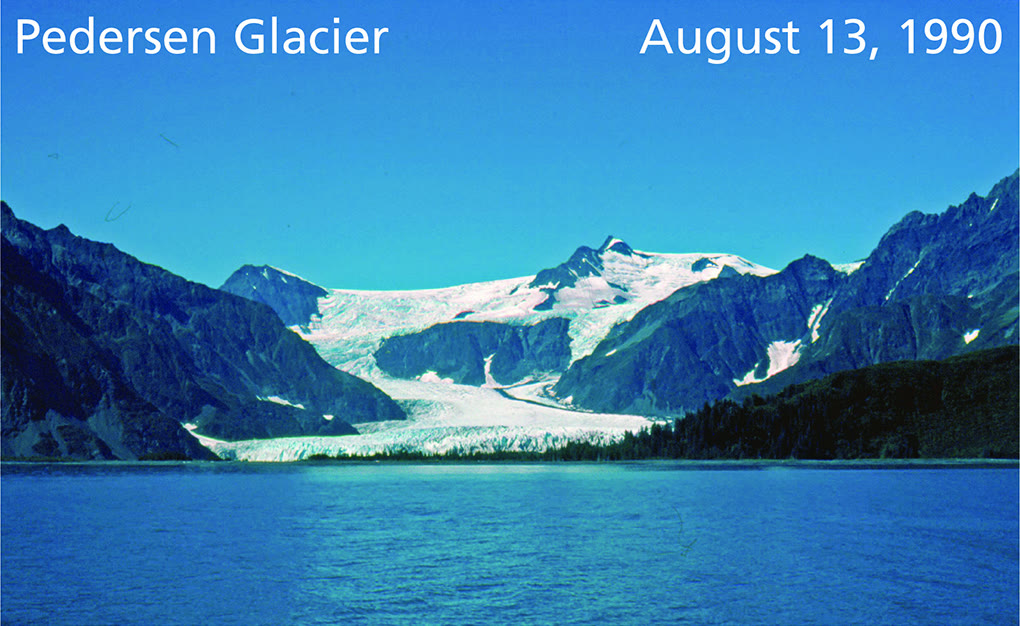
\includegraphics[width=\linewidth]{images/book1/g8-pedersen-1990.jpg}
\end{minipage}\hfill
\begin{minipage}[t]{0.49\linewidth}\centering
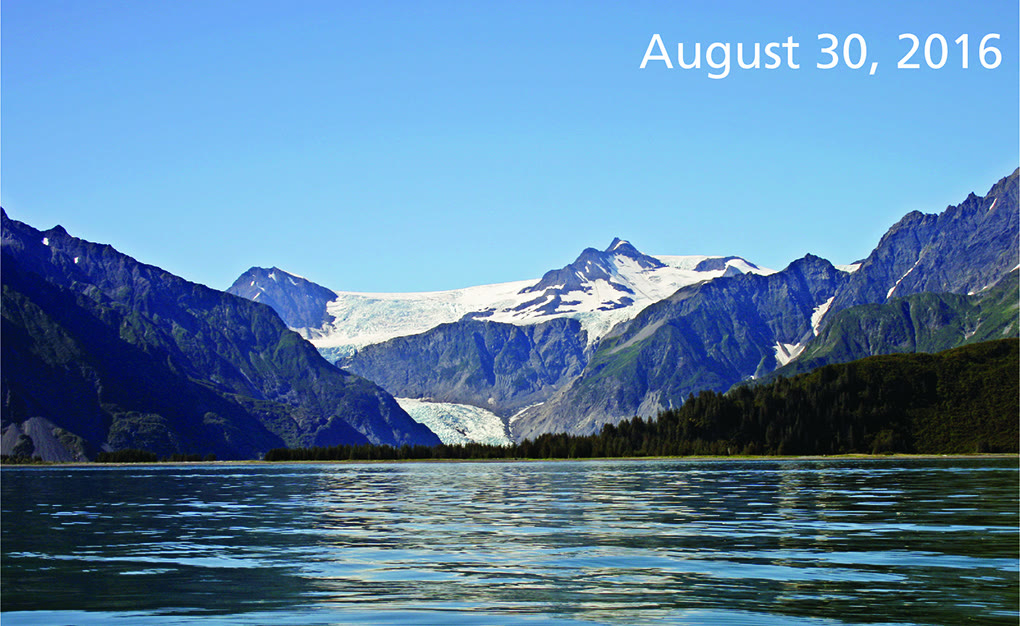
\includegraphics[width=\linewidth]{images/book1/g8-pedersen-2016.jpg}
\end{minipage}

\smallskip
{\small El \omterm{def:g8:ice-on-earth:glacier}{glaciar} Pedersen, en el Parque Nacional Kenai Fjords, Alaska,
visto desde el mismo lugar el 13~de agosto de 1990 (izquierda, fotografía
de M.~Tetreau) y el 30~de agosto de 2016 (derecha, fotografía de
D.~Kurtz). U.S. National Park Service, dominio público (vía Wikimedia
Commons).}
% ledger: commons:pedersen
\label{fig:g8:ice-on-earth:pedersen}
\end{omfigure}

El hielo cubre hoy alrededor de una décima parte de las tierras emergidas.
Se encuentra en los \omterm{def:g1:landscapes-around-us:landform}{valles} de \omterm{def:g1:landscapes-around-us:landform}{montaña}, en dos \omterm{def:g8:ice-on-earth:ice-sheet}{inlandsis} inmensos sobre la
Antártida y Groenlandia, sobre los \omterm{def:g2:water-on-earth:ocean}{mares} polares y, oculto, dentro del
suelo helado del extremo norte. Este capítulo los examina uno por uno,
estudia cómo modela el hielo el terreno y recuerda las épocas en que el
hielo cubría una parte de la Tierra mucho mayor que hoy.
% ledger: nsidc:ice-cover

\begin{recall}
La \omterm{def:g4:clouds-rain-snow:precipitation}{nieve} es una forma de \omterm{def:g4:clouds-rain-snow:precipitation}{precipitación}: cristales de hielo que crecen en
una \omterm{def:g4:clouds-rain-snow:cloud}{nube} y caen sin fundirse (\cref{ch:g4:clouds-rain-snow}). El agua que
corre erosiona el terreno, se lleva los pedazos y los deposita más abajo;
un \omterm{def:g1:landscapes-around-us:water}{río} excava un \omterm{def:g1:landscapes-around-us:landform}{valle} (\cref{ch:g5:water-shapes-the-land}). Cuando el agua
del \omterm{def:g2:water-on-earth:ocean}{mar} se congela, la sal se queda en el agua que rodea el hielo
(\cref{ch:g8:the-oceans}). En física se aprende que el agua se dilata al
congelarse, de modo que el hielo es menos denso que el agua líquida, y que
un cuerpo más ligero que el agua que desplaza flota.
\end{recall}

\section{Los glaciares}

En lo alto de las \omterm{def:g1:landscapes-around-us:landform}{montañas} cae en invierno más \omterm{def:g4:clouds-rain-snow:precipitation}{nieve} de la que se funde en
verano. Año tras año, la \omterm{def:g4:clouds-rain-snow:precipitation}{nieve} nueva entierra la \omterm{def:g4:clouds-rain-snow:precipitation}{nieve} vieja y la
comprime. Los cristales se apelmazan, el aire que había entre ellos es
expulsado y, al cabo de alrededor de un año, la \omterm{def:g4:clouds-rain-snow:precipitation}{nieve} se ha convertido en
\emph{neviza}, un material granuloso, a medio camino entre la \omterm{def:g4:clouds-rain-snow:precipitation}{nieve} y el
hielo. Enterrada cada vez más hondo, la neviza se transforma en hielo
duro y compacto; en la mayoría de los \omterm{def:g8:ice-on-earth:glacier}{glaciares}, esto lleva más de cien
años.
% ledger: nsidc:firn

\begin{definition}[Glaciar]\label{def:g8:ice-on-earth:glacier}
Un \emph{glaciar}\index{glaciar} es una masa de hielo, formada por \omterm{def:g4:clouds-rain-snow:precipitation}{nieve}
acumulada a lo largo de muchos años, que se desplaza lentamente cuesta
abajo sobre el terreno por su propio peso.
\end{definition}
% ledger: nsidc:glacier-def

Un \omterm{def:g8:ice-on-earth:glacier}{glaciar} tiene dos partes. En su parte alta, la \emph{zona de
acumulación}, cae cada año más \omterm{def:g4:clouds-rain-snow:precipitation}{nieve} de la que se funde: el \omterm{def:g8:ice-on-earth:glacier}{glaciar} gana
hielo. En su parte baja, la \emph{zona de ablación}, cada año se funde más
hielo del que cae en forma de \omterm{def:g4:clouds-rain-snow:precipitation}{nieve}: el \omterm{def:g8:ice-on-earth:glacier}{glaciar} pierde hielo. El hielo
ganado arriba no deja de bajar para reemplazar el hielo perdido abajo. Si
las dos cosas se equilibran, la parte delantera del \omterm{def:g8:ice-on-earth:glacier}{glaciar}, su
\emph{frente}, se queda en el mismo lugar.
% ledger: nsidc:glacier-zones

\begin{omfigure}
\begin{tikzpicture}[font=\footnotesize, >={Stealth[length=2mm]}, xscale=1.08]
  % bedrock
  \fill[black!13] (0,4.6) -- (2,3.9) -- (4,3.0) -- (6,2.0) -- (8,1.1)
    -- (10,0.45) -- (11,0.3) -- (13,0.15) -- (13,-0.5) -- (0,-0.5) -- cycle;
  % the ice body, two zones
  \begin{scope}
    \clip (0,5.5) -- (2,4.9) -- (4,4.0) -- (6,2.9) -- (8,1.8) -- (9.4,0.95)
      -- (10,0.45) -- (8,1.1) -- (6,2.0) -- (4,3.0) -- (2,3.9) -- (0,4.6) -- cycle;
    \fill[omIce] (0,-1) rectangle (5,6);
    \fill[omSea!85] (5,-1) rectangle (11,6);
  \end{scope}
  \draw[black!60] (0,5.5) -- (2,4.9) -- (4,4.0) -- (6,2.9) -- (8,1.8)
    -- (9.4,0.95) -- (10,0.45);
  \draw[black!70, line width=0.6pt] (0,4.6) -- (2,3.9) -- (4,3.0) -- (6,2.0)
    -- (8,1.1) -- (10,0.45) -- (11,0.3) -- (13,0.15);
  % snowline
  \draw[dashed, black!70] (5,2.5) -- (5,4.15);
  \node[anchor=south] at (5,4.15) {nevada = fusión};
  % snowflakes and melting
  \foreach \x/\y in {0.5/6.1, 1.3/5.8, 2.1/5.5, 2.9/5.1, 3.7/4.8, 0.9/6.6, 1.7/6.3, 2.5/6.0, 3.3/5.6, 4.1/5.2}
    \node[omCold] at (\x,\y) {$\ast$};
  \foreach \x/\y in {6.4/2.8, 7.2/2.35, 8.0/1.9}
    \draw[omWarm, decorate, decoration={snake, amplitude=0.6mm, segment length=2mm}] (\x,\y) -- ++(0,0.6);
  % flow arrows inside the ice
  \draw[->, omDef, line width=0.9pt] (1.0,4.72) -- (2.2,4.30);
  \draw[->, omDef, line width=0.9pt] (3.0,3.95) -- (4.2,3.41);
  \draw[->, omDef, line width=0.9pt] (5.2,2.88) -- (6.4,2.28);
  \draw[->, omDef, line width=0.9pt] (7.2,1.84) -- (8.3,1.35);
  % moraine and meltwater
  \fill[omLithCongl] (10.15,0.42) .. controls (10.5,0.95) and (10.9,0.95) .. (11.2,0.29) -- cycle;
  \draw[omSea!60!black, line width=1.6pt] (10.05,0.38) .. controls (10.6,0.22) and (11.4,0.12) .. (12.9,0.08);
  % labels
  \node[align=center] at (1.9,7.15) {zona de acumulación:\\ la nieve se acumula, el glaciar gana hielo};
  \node[align=center] at (10.0,3.3) {zona de ablación:\\ el hielo se funde, el glaciar pierde hielo};
  \node[align=left, anchor=west, omDef] at (4.4,1.3) {el hielo fluye\\ cuesta abajo};
  \draw[black!60] (10.0,0.5) -- (9.6,-0.1) node[below] {frente};
  \draw[black!60] (10.7,0.85) -- (11.3,1.4) node[above] {morrena};
  \node[anchor=north east] at (12.9,0.0) {torrente de agua de fusión};
  \node at (2.2,2.6) {roca madre};
\end{tikzpicture}

{\small Un \omterm{def:g8:ice-on-earth:glacier}{glaciar} de \omterm{def:g1:landscapes-around-us:landform}{valle} visto en sección longitudinal (un esquema, no a
escala). Por encima de la línea discontinua, la \omterm{def:g4:clouds-rain-snow:precipitation}{nieve} se acumula más
deprisa de lo que se funde; por debajo, el hielo se funde más deprisa de lo
que cae la \omterm{def:g4:clouds-rain-snow:precipitation}{nieve}. El hielo fluye de una parte a la otra.}
\label{fig:g8:ice-on-earth:long-section}
\end{omfigure}

¿Cómo puede fluir el hielo, que es sólido? Bajo el peso del hielo que
tiene encima, el hielo profundo de un \omterm{def:g8:ice-on-earth:glacier}{glaciar} se deforma lentamente, igual
que se extiende una capa gruesa de miel fría. El \omterm{def:g8:ice-on-earth:glacier}{glaciar} también se
desliza sobre la \omterm{def:g3:stones-pebbles-sand:rock}{roca} de debajo, sobre una fina película de agua o sobre
\omterm{def:g3:stones-pebbles-sand:sand}{barro} húmedo. La base del \omterm{def:g8:ice-on-earth:glacier}{glaciar}, que roza contra la \omterm{def:g3:stones-pebbles-sand:rock}{roca}, avanza más
despacio que su superficie. La mayoría de los \omterm{def:g8:ice-on-earth:glacier}{glaciares} se mueven de forma
lenta y regular; unos pocos \emph{se aceleran} de repente. En 1986, el
\omterm{def:g8:ice-on-earth:glacier}{glaciar} Hubbard, en Alaska, avanzó bruscamente unos \qty{10}{m} al día, y
el avance más rápido registrado, el del \omterm{def:g8:ice-on-earth:glacier}{glaciar} Kutiah, en Pakistán, en
1953, fue de unos \qty{112}{m} al día de media durante tres meses.
% ledger: nsidc:glacier-flow, nsidc:surges

Cuando un \omterm{def:g8:ice-on-earth:glacier}{glaciar} pierde más hielo abajo del que gana arriba, su frente
retrocede \omterm{def:g1:landscapes-around-us:landform}{valle} arriba: el \omterm{def:g8:ice-on-earth:glacier}{glaciar} \emph{retrocede}. Un \omterm{def:g8:ice-on-earth:glacier}{glaciar} en
retroceso sigue fluyendo cuesta abajo, como una cinta transportadora;
simplemente se funde más deprisa de lo que fluye. El \omterm{def:g8:ice-on-earth:glacier}{glaciar} Muir, en
Alaska, llenaba todo su \omterm{def:g1:landscapes-around-us:landform}{valle} hasta el \omterm{def:g2:water-on-earth:ocean}{mar} en 1941. En 2004, su frente
había retrocedido \qty{12}{km}, y la superficie del hielo había bajado más
de \qty{800}{m}.
% ledger: nsidc:glacier-flow, nsidc:muir

\section{Cómo modela el hielo un valle}

Un \omterm{def:g8:ice-on-earth:glacier}{glaciar} es una poderosa herramienta de \omterm{def:g5:water-shapes-the-land:erosion}{erosión}. Su hielo se congela
sobre bloques de \omterm{def:g3:stones-pebbles-sand:rock}{roca} suelta y los arranca; las piedras que lleva
incrustadas en la base raspan la \omterm{def:g3:stones-pebbles-sand:rock}{roca} de debajo como una lija. El \omterm{def:g8:ice-on-earth:glacier}{glaciar}
transporta toda esa \omterm{def:g3:stones-pebbles-sand:rock}{roca}, desde el polvo fino hasta bloques enormes, \omterm{def:g1:landscapes-around-us:landform}{valle}
abajo como una cinta transportadora, y la deja donde el hielo se funde.
% ledger: nps:u-valley

\begin{omfigure}
\begin{tikzpicture}[font=\footnotesize, >={Stealth[length=2mm]}]
  % V-shaped valley
  \fill[black!13] (0,3) -- (2.1,0.35) -- (2.5,0.35) -- (4.6,3) -- (4.6,-0.4) -- (0,-0.4) -- cycle;
  \draw[black!70, line width=0.6pt] (0,3) -- (2.1,0.35) -- (2.5,0.35) -- (4.6,3);
  \fill[omSea] (2.1,0.35) -- (2.5,0.35) -- (2.42,0.2) -- (2.18,0.2) -- cycle;
  \node[align=center] at (2.3,-0.85) {un río excava un valle\\ estrecho en forma de V};
  % arrow
  \draw[->, line width=1pt] (5.0,1.5) -- (6.2,1.5) node[midway, above, align=center] {un glaciar\\ lo llena};
  % U-shaped valley
  \begin{scope}[xshift=6.6cm]
    \fill[black!13] (0,3) .. controls (0.6,1.0) and (0.9,0.25) .. (1.6,0.2)
      -- (3.0,0.2) .. controls (3.7,0.25) and (4.0,1.0) .. (4.6,3) -- (4.6,-0.4) -- (0,-0.4) -- cycle;
    \draw[black!70, line width=0.6pt] (0,3) .. controls (0.6,1.0) and (0.9,0.25) .. (1.6,0.2)
      -- (3.0,0.2) .. controls (3.7,0.25) and (4.0,1.0) .. (4.6,3);
    \draw[dashed, black!40] (0,3) -- (2.1,0.35) -- (2.5,0.35) -- (4.6,3);
    \draw[omCold, line width=0.9pt] (0.37,2.2) -- (4.23,2.2);
    \node[omCold, anchor=south, font=\scriptsize] at (2.3,2.2) {antigua superficie del hielo};
    \fill[omLithCongl] (0.75,0.95) .. controls (0.95,1.2) and (1.1,1.1) .. (1.2,0.6) -- cycle;
    \fill[omLithCongl] (3.85,0.95) .. controls (3.65,1.2) and (3.5,1.1) .. (3.4,0.6) -- cycle;
    \node[align=center] at (2.3,-0.85) {cuando el hielo ha desaparecido: un ancho\\ valle en forma de U, de laderas empinadas};
    \draw[black!60] (3.65,0.95) -- (4.85,0.6) node[right, align=left] {morrena\\ lateral};
    \node[font=\scriptsize, black!55, align=center] at (2.3,1.6) {(la antigua V,\\ en discontinua)};
  \end{scope}
\end{tikzpicture}

{\small El mismo \omterm{def:g1:landscapes-around-us:landform}{valle} de \omterm{def:g1:landscapes-around-us:landform}{montaña} en sección transversal, antes y después
de un \omterm{def:g8:ice-on-earth:glacier}{glaciar} (un esquema). El hielo transforma el estrecho \omterm{def:g1:landscapes-around-us:landform}{valle} fluvial
en una artesa ancha, de fondo amplio y laderas empinadas, y deja a lo largo
de sus bordes unas crestas de derrubios de \omterm{def:g3:stones-pebbles-sand:rock}{roca}.}
\label{fig:g8:ice-on-earth:v-and-u}
\end{omfigure}

\begin{definition}[Valle en U y morrena]\label{def:g8:ice-on-earth:glacial-landforms}
Un \emph{valle en U}\index{valle en U} es un \omterm{def:g1:landscapes-around-us:landform}{valle} de fondo ancho y plano y
laderas empinadas, excavado por un \omterm{def:g8:ice-on-earth:glacier}{glaciar} que ensanchó y profundizó un
estrecho \omterm{def:g1:landscapes-around-us:landform}{valle} fluvial en forma de V. Una \emph{morrena}\index{morrena} es
una cresta de derrubios de \omterm{def:g3:stones-pebbles-sand:rock}{roca}, desde polvo hasta bloques, dejada por un
\omterm{def:g8:ice-on-earth:glacier}{glaciar}: una \emph{morrena lateral} a lo largo de su borde, una
\emph{morrena frontal} en su extremo.
\end{definition}
% ledger: usgs:erratic, nps:u-valley, nps:moraines

Las \omterm{def:g8:ice-on-earth:glacial-landforms}{morrenas} son pistas útiles. Una \omterm{def:g8:ice-on-earth:glacial-landforms}{morrena} frontal muy abajo en un \omterm{def:g1:landscapes-around-us:landform}{valle},
sin hielo por ninguna parte cerca de ella, muestra hasta dónde llegó el
\omterm{def:g8:ice-on-earth:glacier}{glaciar}; una \omterm{def:g8:ice-on-earth:glacial-landforms}{morrena} lateral muy alta en la ladera de un \omterm{def:g1:landscapes-around-us:landform}{valle} muestra qué
espesor llegó a tener el hielo. Un gran bloque que descansa solo en un
campo, hecho de una \omterm{def:g3:stones-pebbles-sand:rock}{roca} que no se encuentra en ningún lugar cercano, es
otra pista: es un \emph{bloque errático}, una \omterm{def:g3:stones-pebbles-sand:rock}{roca} transportada lejos de
su lugar de origen por un \omterm{def:g8:ice-on-earth:glacier}{glaciar} y abandonada cuando el hielo se fundió.
Los bloques erráticos van desde \omterm{def:g3:stones-pebbles-sand:pebble}{cantos rodados} hasta bloques más grandes
que una casa.
% ledger: nps:moraines, usgs:erratic

\begin{inthefield}[Leer un valle modelado por el hielo]
En una excursión por la \omterm{def:g1:landscapes-around-us:landform}{montaña}, o en una fotografía de un \omterm{def:g1:landscapes-around-us:landform}{valle} de
\omterm{def:g1:landscapes-around-us:landform}{montaña}, observa la forma del \omterm{def:g1:landscapes-around-us:landform}{valle} en sección transversal: ¿una V
estrecha, o una U ancha de paredes empinadas? Busca en el fondo del \omterm{def:g1:landscapes-around-us:landform}{valle}
largas crestas de piedras y tierra revueltas que corran a lo largo de sus
laderas o lo atraviesen: pueden ser \omterm{def:g8:ice-on-earth:glacial-landforms}{morrenas}. Busca grandes bloques que no
coincidan con la \omterm{def:g3:stones-pebbles-sand:rock}{roca} de alrededor, y superficies de \omterm{def:g3:stones-pebbles-sand:rock}{roca} lisas rayadas
por largas líneas paralelas. No te salgas de los caminos, mantente lejos
de los bordes de las pendientes empinadas y del propio hielo, y dibuja lo
que veas en tu cuaderno.
\end{inthefield}

\section{Inlandsis, plataformas de hielo e icebergs}

Las mayores masas de hielo de la Tierra no están en los \omterm{def:g1:landscapes-around-us:landform}{valles} de \omterm{def:g1:landscapes-around-us:landform}{montaña}:
cubren regiones enteras. El \omterm{def:g8:ice-on-earth:ice-sheet}{inlandsis} antártico se extiende sobre
casi \num{14}~millones de~\unit{km^2} y tiene casi \qty{4.9}{km} de espesor
en su punto más grueso. El \omterm{def:g8:ice-on-earth:ice-sheet}{inlandsis} de Groenlandia cubre unos
\num{1.7}~millones de~\unit{km^2}, cuatro quintas partes de la isla, y
tiene más de \qty{3}{km} de espesor. Juntos contienen más del 99~\% del
hielo continental, y más de dos tercios de toda el \omterm{def:g2:water-on-earth:salt-fresh}{agua dulce} de la Tierra.
% ledger: nsidc:ice-sheets

\begin{definition}[Inlandsis, plataforma de hielo e iceberg]\label{def:g8:ice-on-earth:ice-sheet}
Un \emph{inlandsis}\index{inlandsis} es una masa de hielo que
cubre más de \qty{50000}{km^2} de tierra, como una cúpula inmensa que se
extiende hacia fuera en todas direcciones. Donde el hielo que fluye desde
la tierra llega al \omterm{def:g2:water-on-earth:ocean}{mar} y sigue flotando sobre él, todavía unido al hielo
de detrás, forma una \emph{plataforma de hielo}\index{plataforma de hielo}.
Un \emph{iceberg}\index{iceberg} es un gran bloque de hielo, de más de
\qty{5}{m} de ancho, que se ha desprendido de un \omterm{def:g8:ice-on-earth:glacier}{glaciar} o de una
plataforma de hielo y flota en el \omterm{def:g2:water-on-earth:ocean}{mar}.
\end{definition}
% ledger: nsidc:ice-sheets, nsidc:ice-shelves, nsidc:iceberg

\begin{omfigure}
\begin{minipage}[c]{0.5\linewidth}\centering
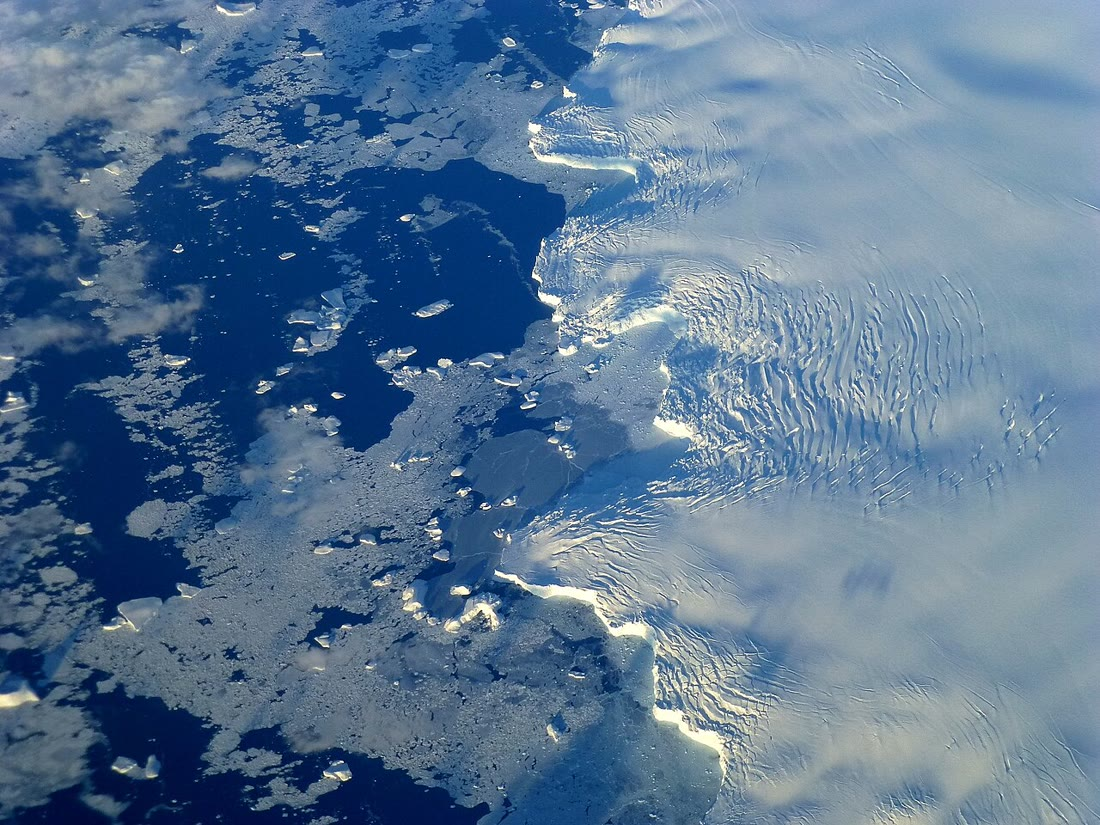
\includegraphics[width=\linewidth]{images/book1/g8-ice-shelf-edge.jpg}
\end{minipage}\hfill
\begin{minipage}[c]{0.46\linewidth}\raggedright
{\small El borde de una \omterm{def:g8:ice-on-earth:ice-sheet}{plataforma de hielo} cerca de la isla Adelaida,
frente a la península Antártica, visto desde un avión el 28~de octubre de
2012. El hielo blanco, grueso y arrugado de la derecha es la \omterm{def:g8:ice-on-earth:ice-sheet}{plataforma de
hielo}; a la izquierda, trozos rotos de \omterm{def:g8:ice-on-earth:sea-ice}{hielo marino} más fino flotan sobre
el agua oscura. NASA, Operation IceBridge (dominio público, vía Wikimedia
Commons).}
\end{minipage}
% ledger: commons:ice-shelf
\label{fig:g8:ice-on-earth:ice-shelf}
\end{omfigure}

El agua retenida en los \omterm{def:g8:ice-on-earth:ice-sheet}{inlandsis} procede del \omterm{def:g2:water-on-earth:ocean}{océano}: se evaporó,
cayó en forma de \omterm{def:g4:clouds-rain-snow:precipitation}{nieve} y se acumuló en tierra firme. Si se fundiera todo el
hielo de Groenlandia, el \omterm{def:g2:water-on-earth:ocean}{mar} subiría unos \qty{7.4}{m}; si se fundiera todo
el hielo de la Antártida, unos \qty{58}{m}. Todos los \omterm{def:g8:ice-on-earth:glacier}{glaciares} de \omterm{def:g1:landscapes-around-us:landform}{montaña}
del mundo, más de \num{200000}, añadirían menos de medio metro.
% ledger: nsidc:ice-sheets, nsidc:ice-cover

\begin{omfigure}
\begin{tikzpicture}
\begin{axis}[omrecord, xbar, width=10.5cm, height=3.6cm, xmin=0, xmax=68,
  bar width=9pt, ytick=data, symbolic y coords={glaciares,Groenlandia,Antartida},
  yticklabels={todos los glaciares de montaña, inlandsis de Groenlandia, inlandsis antártico},
  xlabel={subida del mar si se fundiera todo (m)}, enlarge y limits=0.3,
  nodes near coords, nodes near coords style={font=\footnotesize, anchor=west, fill=white, inner sep=1.5pt},
  ymajorgrids=false]
  \addplot[fill=omIce!80!black, draw=black!60] coordinates {(0.5,glaciares) (7.4,Groenlandia) (58,Antartida)};
\end{axis}
\end{tikzpicture}

{\small Cuánto subiría el \omterm{def:g2:water-on-earth:ocean}{mar} si cada tipo de hielo continental se fundiera
por completo (valores del National Snow and Ice Data Center; el valor de
los \omterm{def:g8:ice-on-earth:glacier}{glaciares} es un límite superior, ``algo menos de medio metro'').}
% ledger: nsidc:ice-sheets, nsidc:ice-cover
\label{fig:g8:ice-on-earth:sea-level-bars}
\end{omfigure}

El hielo flotante es distinto. Una \omterm{def:g8:ice-on-earth:ice-sheet}{plataforma de hielo} o un \omterm{def:g8:ice-on-earth:ice-sheet}{iceberg} ya
flotan en el \omterm{def:g2:water-on-earth:ocean}{mar}: ya han desplazado su propio peso de agua. Cuando se
rompen o se funden, el \omterm{def:g2:water-on-earth:ocean}{mar} no sube. Pero una \omterm{def:g8:ice-on-earth:ice-sheet}{plataforma de hielo} retiene
los \omterm{def:g8:ice-on-earth:glacier}{glaciares} que tiene detrás, como un tapón en una botella; cuando la
\omterm{def:g8:ice-on-earth:ice-sheet}{plataforma de hielo} Larsen~B, en la Antártida, se desintegró en 2002, los
\omterm{def:g8:ice-on-earth:glacier}{glaciares} que tenía detrás se aceleraron, algunos hasta ocho veces su
velocidad anterior, y vertieron más hielo continental en el \omterm{def:g2:water-on-earth:ocean}{mar}.
% ledger: nsidc:ice-shelves

\begin{inthelab}[Hielo flotante y hielo sobre tierra]
En el interior, pon una piedra pequeña en cada uno de dos vasos
transparentes, de modo que sobresalga del agua cuando los llenes. En el
primer vaso, haz flotar unos cubitos de hielo sobre el agua. En el
segundo, coloca el mismo número de cubitos sobre la piedra, fuera del
agua. Llena los dos vasos de agua hasta el mismo nivel y márcalo con un
rotulador. Espera a que se haya fundido todo el hielo y compara después
los niveles del agua con las marcas. ¿Qué vaso se comporta como el \omterm{def:g2:water-on-earth:ocean}{mar}
cuando se funde un \omterm{def:g8:ice-on-earth:ice-sheet}{iceberg}, y cuál como el \omterm{def:g2:water-on-earth:ocean}{mar} cuando se funde un
\omterm{def:g8:ice-on-earth:ice-sheet}{inlandsis}?
\end{inthelab}

\section{El hielo marino}

El \omterm{def:g8:ice-on-earth:sea-ice}{hielo marino} es otra cosa: es el propio \omterm{def:g2:water-on-earth:ocean}{mar}, congelado. Cada invierno,
la superficie de los \omterm{def:g2:water-on-earth:ocean}{océanos} polares se congela sobre una extensión
inmensa; cada verano, buena parte de ese hielo vuelve a fundirse. En el
Ártico, el hielo es mínimo al final del verano, en septiembre, y máximo al
final del invierno, en marzo. Los satélites han medido su
\emph{extensión}, la superficie de \omterm{def:g2:water-on-earth:ocean}{mar} en la que al menos el 15~\% de la
superficie está cubierta de hielo, cada día desde finales de la década de
1970.
% ledger: nsidc:sea-ice-def

\begin{definition}[Hielo marino]\label{def:g8:ice-on-earth:sea-ice}
El \emph{hielo marino}\index{hielo marino} es agua de \omterm{def:g2:water-on-earth:ocean}{mar} congelada: se
forma, crece y se funde en el propio \omterm{def:g2:water-on-earth:ocean}{océano}. Es distinto de los \omterm{def:g8:ice-on-earth:ice-sheet}{icebergs} y
de las \omterm{def:g8:ice-on-earth:ice-sheet}{plataformas de hielo}, que flotan en el \omterm{def:g2:water-on-earth:ocean}{mar} pero están hechos de
\omterm{def:g4:clouds-rain-snow:precipitation}{nieve} caída sobre tierra firme.
\end{definition}
% ledger: nsidc:sea-ice-def

El \omterm{def:g8:ice-on-earth:sea-ice}{hielo marino} importa mucho más allá de los \omterm{def:g3:continents-and-oceans:poles}{polos}. El agua de \omterm{def:g2:water-on-earth:ocean}{mar} libre
es oscura: solo refleja alrededor del 6~\% de la luz solar que le llega y
absorbe el resto. El \omterm{def:g8:ice-on-earth:sea-ice}{hielo marino} refleja del 50 al 70~\%, y el \omterm{def:g8:ice-on-earth:sea-ice}{hielo
marino} cubierto de \omterm{def:g4:clouds-rain-snow:precipitation}{nieve}, hasta el 90~\%. Cuando el hielo se funde, el agua
oscura de debajo absorbe más energía del Sol y se calienta, lo que funde
más hielo.
% ledger: nsidc:sea-ice-reflect

\begin{omfigure}
\begin{tikzpicture}
\begin{axis}[omrecord, width=13cm, height=5.4cm, xmin=1977, xmax=2027,
  ymin=3, ymax=8.2, xtick={1980,1990,...,2020},
  x tick label style={/pgf/number format/1000 sep={}},
  xlabel={año}, ylabel={extensión (millones de km$^2$)},
  legend style={at={(0.98,0.97)}, anchor=north east, draw=none, fill=white}]
  \addplot[omCold, mark=*, mark size=1.3pt, line width=0.6pt]
    table[x=year, y=extent_Mkm2] {figdata/out/grade-8-sea_ice-extent.dat};
  \addlegendentry{extensión media de septiembre}
  \addplot[omWarm, dashed, line width=1pt]
    table[x=year, y=extent_Mkm2] {figdata/out/grade-8-sea_ice-trend.dat};
  \addlegendentry{línea de tendencia}
  \node[font=\scriptsize, anchor=north] at (axis cs:2012,3.5) {2012};
\end{axis}
\end{tikzpicture}

{\small La extensión del \omterm{def:g8:ice-on-earth:sea-ice}{hielo marino} ártico cada mes de septiembre,
1979--2025, y la recta que mejor sigue los puntos. Datos: NSIDC Sea Ice
Index, versión~4 (F.~Fetterer y otros, 2025).}
% ledger: data:b1-nsidc-sea-ice (figdata/grade-8/sea_ice.py)
\label{fig:g8:ice-on-earth:sea-ice}
\end{omfigure}

Los puntos suben y bajan de un año a otro: el \omterm{def:g1:watching-the-weather:weather}{tiempo} de cada verano
cuenta. Pero a lo largo de los años bajan claramente. Para ver el cambio a
través de los altibajos, los científicos trazan una \emph{línea de
tendencia}, la recta que pasa lo más cerca posible de todos los puntos.
% ledger: data:b1-nsidc-sea-ice (figdata/grade-8/sea_ice.py)

\begin{method}[Leer una tendencia en un gráfico]
\begin{enumerate}
  \item Lee los ejes: qué se mide, en qué unidad, a lo largo de qué años.
  \item Observa los puntos: ¿hay una subida general, una bajada general, o
        ninguna de las dos, detrás de los altibajos?
  \item Lee la línea de tendencia en el primer año y en el último.
  \item Calcula la diferencia y divídela entre el número de años (o de
        décadas) que los separan: es el cambio medio por año (o por
        década).
  \item No le des demasiada importancia a un solo año: un punto aislado
        lejos de la línea es el \omterm{def:g1:watching-the-weather:weather}{tiempo} meteorológico; la línea es la
        tendencia.
\end{enumerate}
\end{method}

\begin{example}[El hielo de septiembre del Ártico]
En el gráfico, la línea de tendencia está en unos
\num{7.6}~millones de~\unit{km^2} en 1979 y en unos
\num{4.1}~millones de~\unit{km^2} en 2025. El cambio es de $7.6 - 4.1 =
3.5$ millones de km$^2$ en $2025 - 1979 = 46$ años, es decir, 4.6 décadas:
$3.5 \div 4.6 \approx 0.76$. El \omterm{def:g8:ice-on-earth:sea-ice}{hielo marino} de septiembre ha disminuido
unos \num{0.76}~millones de~\unit{km^2} por década: en 46 años, la línea
de tendencia ha perdido casi la mitad de su valor de 1979. El punto más
bajo, \num{3.57}~millones de~\unit{km^2} en 2012, queda muy por debajo de
la línea: aquel verano fue excepcional.
\end{example}
% ledger: data:b1-nsidc-sea-ice (figdata/grade-8/sea_ice.py), nsidc:sea-ice-reflect

Las medidas muestran que el \omterm{def:g8:ice-on-earth:sea-ice}{hielo marino} de verano del Ártico se ha vuelto
a la vez más pequeño y más fino desde la década de 1980, a medida que el
Ártico se ha calentado. El \cref{ch:g9:climate-past-and-present} estudia
cómo está cambiando el \omterm{def:g5:weather-and-climate:climate}{clima} de la Tierra, y por qué.
% ledger: nsidc:sea-ice-reflect

\section{El permafrost}

En el extremo norte, el frío penetra muy hondo en el suelo. Bajo la
tundra de América del Norte, de Groenlandia y del norte de Asia, el suelo
y la \omterm{def:g3:stones-pebbles-sand:rock}{roca} permanecen helados todo el año, y a menudo llevan miles de años
helados. Solo una fina capa superior, la \emph{capa activa}, se deshiela
cada verano y vuelve a helarse cada invierno; en ella crecen las plantas,
y el agua, que no puede filtrarse hacia el suelo helado de debajo, forma
charcas en la superficie.
% ledger: nsidc:permafrost

\begin{definition}[Permafrost]\label{def:g8:ice-on-earth:permafrost}
El \emph{permafrost}\index{permafrost} es un terreno, suelo o \omterm{def:g3:stones-pebbles-sand:rock}{roca}, que
permanece a \qty{0}{\degreeCelsius} o por debajo durante al menos dos años
seguidos.
\end{definition}
% ledger: nsidc:permafrost

El \omterm{def:g8:ice-on-earth:permafrost}{permafrost} se extiende bajo unos \num{23}~millones de~\unit{km^2}, una
cuarta parte de las tierras emergidas del \omterm{def:g3:continents-and-oceans:equator}{hemisferio norte}, y bajo
alrededor del 85~\% de Alaska. Un suelo helado lleno de hielo es tan duro
como la \omterm{def:g3:stones-pebbles-sand:rock}{roca}; cuando su hielo se funde, el suelo se convierte en \omterm{def:g3:stones-pebbles-sand:sand}{barro} y se
hunde. Las carreteras se agrietan, los edificios se inclinan y los
oleoductos pueden romperse: donde atraviesa \omterm{def:g8:ice-on-earth:permafrost}{permafrost}, el oleoducto
Trans-Alaska va por encima del suelo a lo largo de \qty{676}{km}. Al
deshelarse, el \omterm{def:g8:ice-on-earth:permafrost}{permafrost} también deja que se descompongan restos de
plantas congelados en él durante miles de años, que liberan dióxido de
carbono y metano al aire.
% ledger: nsidc:permafrost, nsidc:permafrost-thaw

\begin{omfigure}
\begin{minipage}[c]{0.5\linewidth}\centering
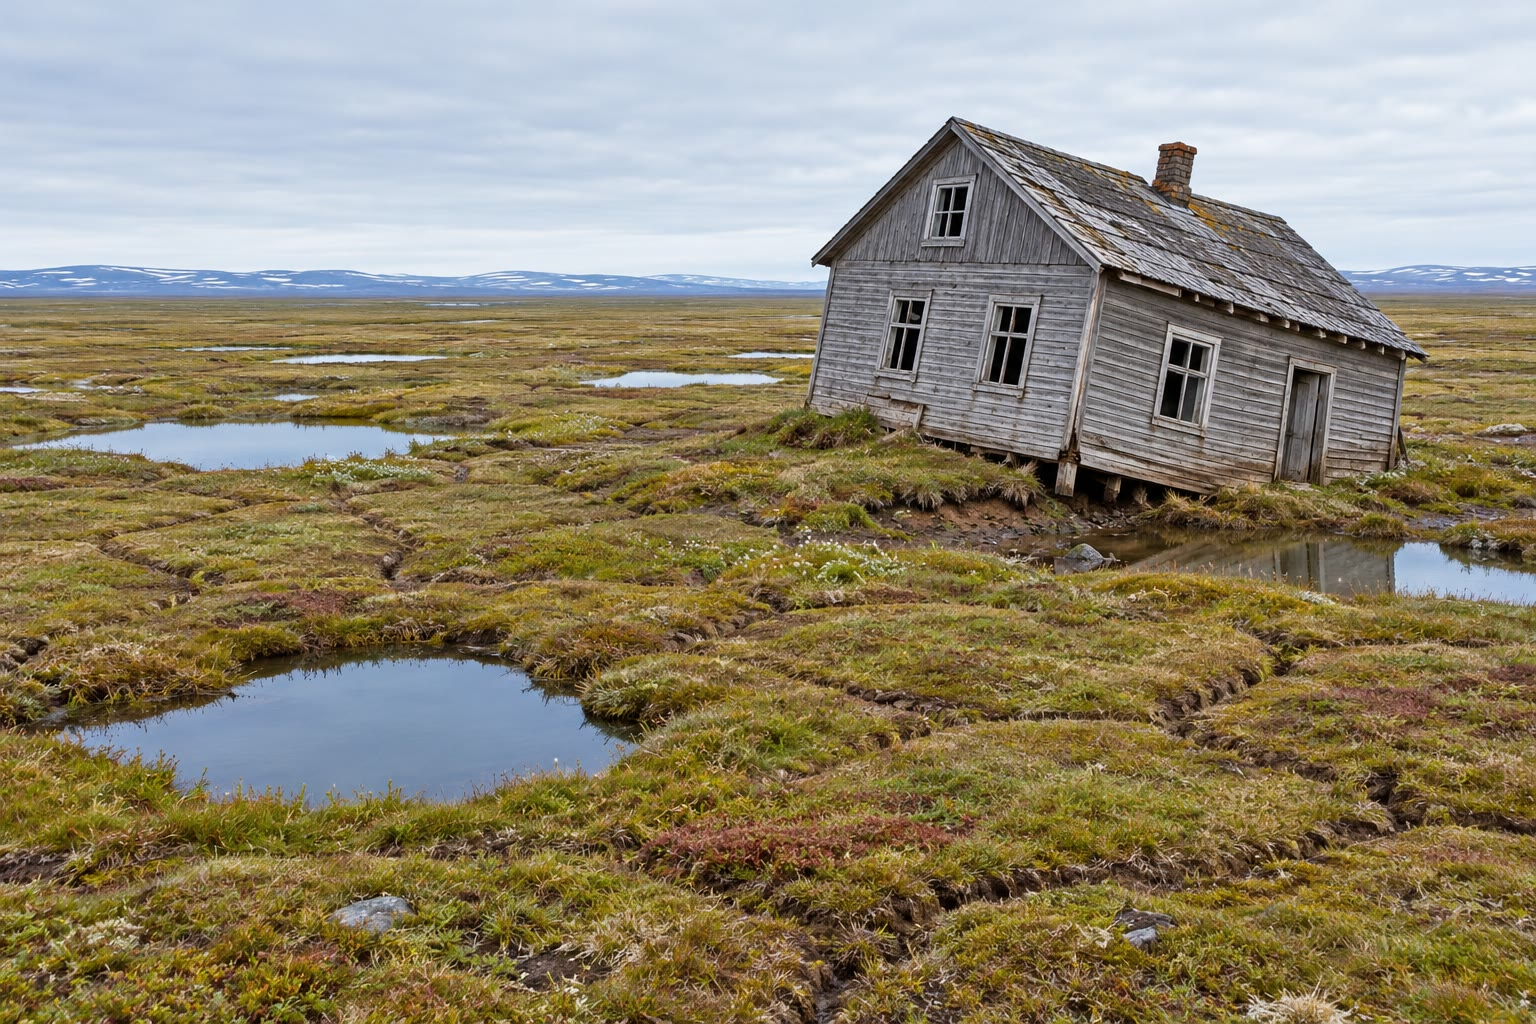
\includegraphics[width=\linewidth]{images/book1/ai/g8-permafrost-house.jpg}
\end{minipage}\hfill
\begin{minipage}[c]{0.46\linewidth}\centering
\begin{tikzpicture}[font=\footnotesize]
  \fill[omLithAlluv] (0,0) rectangle (3.2,-0.6);
  \fill[omIce!70!omLithShale] (0,-0.6) rectangle (3.2,-3.0);
  \foreach \x/\y in {0.4/-1.0, 1.5/-1.3, 2.6/-0.9, 0.9/-1.9, 2.1/-2.2, 0.5/-2.6, 2.8/-2.6}
    \fill[white] (\x,\y) ellipse (0.22 and 0.06);
  \fill[omLithShale!60] (0,-3.0) rectangle (3.2,-3.6);
  \draw[green!45!black, line width=1pt] (0,0) -- (3.2,0);
  \node[anchor=west, align=left] at (3.3,-0.3) {capa activa:\\ se deshiela\\ cada verano};
  \node[anchor=west, align=left] at (3.3,-1.8) {permafrost:\\ helado todo el año,\\ lentejones de hielo};
  \node[anchor=west, align=left] at (3.3,-3.3) {suelo no\\ helado};
\end{tikzpicture}
\end{minipage}

\smallskip
{\small A la izquierda: una casa que se inclina sobre un \omterm{def:g8:ice-on-earth:permafrost}{permafrost} en
deshielo en la tundra (ilustración generada por IA de una escena
genérica). A la derecha: el suelo bajo la tundra (un esquema, no a
escala).}
\label{fig:g8:ice-on-earth:permafrost}
\end{omfigure}

\section{Las glaciaciones}

El hielo no siempre ha cubierto la misma parte de la Tierra. Hace unos
\num{20000} años, unos \omterm{def:g8:ice-on-earth:ice-sheet}{inlandsis} cubrían buena parte de América
del Norte y del norte de Europa, incluida Escandinavia. Los \omterm{def:g8:ice-on-earth:glacier}{glaciares}
cubrían entonces alrededor de una cuarta parte de las tierras emergidas,
frente a una décima parte hoy. Había tanta agua retenida en ese hielo que
el \omterm{def:g2:water-on-earth:ocean}{mar} estaba más de \qty{120}{m} por debajo de su nivel actual: partes de
las \omterm{def:g8:the-oceans:seafloor}{plataformas continentales} de hoy eran tierra firme. A partir de hace
unos \num{15000} años, los \omterm{def:g8:ice-on-earth:ice-sheet}{inlandsis} se fundieron y retrocedieron, y el \omterm{def:g2:water-on-earth:ocean}{mar}
subió; alcanzó aproximadamente su nivel actual hace unos \num{8000} años.
% ledger: usgs:lgm, nsidc:ice-sheets, nsidc:ice-cover

\begin{definition}[Glaciación]\label{def:g8:ice-on-earth:ice-age}
Una \emph{glaciación}\index{glaciacion@glaciación} es un largo periodo
frío de la historia de la Tierra en el que los \omterm{def:g8:ice-on-earth:ice-sheet}{inlandsis} se
extienden mucho más allá de las regiones polares y cubren grandes partes de
los \omterm{def:g3:continents-and-oceans:continent}{continentes}. La última glaciación tuvo su momento más frío hace unos
\num{20000} años y terminó hace unos \num{12000} años.
\end{definition}
% ledger: usgs:lgm, nps:u-valley

Las huellas de la última \omterm{def:g8:ice-on-earth:ice-age}{glaciación} están por todas partes en las tierras
que cubrió: \omterm{def:g8:ice-on-earth:glacial-landforms}{valles en U} lejos de cualquier \omterm{def:g8:ice-on-earth:glacier}{glaciar} actual, \omterm{def:g8:ice-on-earth:glacial-landforms}{morrenas}
frontales que atraviesan \omterm{def:g1:landscapes-around-us:landform}{llanuras}, bloques erráticos en medio de los
campos. Y no fue la única. A lo largo de los últimos cientos de miles de
años, las \omterm{def:g8:ice-on-earth:ice-age}{glaciaciones} y las épocas más cálidas que las separan se han
sucedido una y otra vez; vivimos en una de las épocas cálidas. El
\cref{ch:g9:climate-past-and-present} cuenta cómo leen los científicos esta
larga historia en el propio hielo de la Antártida.
% ledger: nps:u-valley, nps:moraines, usgs:erratic

\section{Ejercicios}

\begin{exercise}[$\star$]\label{exo:g8:ice-on-earth:1}
Con la sección longitudinal de un \omterm{def:g8:ice-on-earth:glacier}{glaciar} de este capítulo, nombra: (a) la
parte del \omterm{def:g8:ice-on-earth:glacier}{glaciar} donde gana hielo; (b) la parte donde pierde hielo; (c) la
parte delantera del \omterm{def:g8:ice-on-earth:glacier}{glaciar}; (d) la cresta de derrubios de \omterm{def:g3:stones-pebbles-sand:rock}{roca} de su
extremo.
\end{exercise}

\begin{exercise}[$\star$]\label{exo:g8:ice-on-earth:2}
% ledger: nsidc:firn, nsidc:glacier-flow, nsidc:sea-ice-def
¿Verdadero o falso? Corrige las frases falsas. (a) Un \omterm{def:g8:ice-on-earth:glacier}{glaciar} está hecho de
agua de \omterm{def:g2:water-on-earth:ocean}{mar} congelada. (b) La \omterm{def:g4:clouds-rain-snow:precipitation}{nieve} tarda alrededor de un año en
convertirse en neviza. (c) Cuando un \omterm{def:g8:ice-on-earth:glacier}{glaciar} retrocede, su hielo fluye
cuesta arriba. (d) En el Ártico, el \omterm{def:g8:ice-on-earth:sea-ice}{hielo marino} es mínimo en septiembre.
\end{exercise}

\begin{exercise}[$\star$]\label{exo:g8:ice-on-earth:3}
% ledger: usgs:erratic, nsidc:permafrost
Da la palabra que corresponde a cada descripción: (a) un \omterm{def:g1:landscapes-around-us:landform}{valle} de fondo
ancho y laderas empinadas, excavado por el hielo; (b) un bloque
transportado lejos de su lugar de origen por un \omterm{def:g8:ice-on-earth:glacier}{glaciar}; (c) una placa de
hielo flotante todavía unida al hielo de tierra firme; (d) un terreno que
permanece helado durante al menos dos años seguidos.
\end{exercise}

\begin{exercise}[$\star$]\label{exo:g8:ice-on-earth:4}
% ledger: nsidc:ice-sheets, nsidc:ice-cover
(a) ¿Qué dos regiones están cubiertas hoy por \omterm{def:g8:ice-on-earth:ice-sheet}{inlandsis}? (b) ¿Cuál
de las dos haría subir más el \omterm{def:g2:water-on-earth:ocean}{mar} si se fundiera todo su hielo, y cuánto?
(c) ¿Qué parte de las tierras emergidas está cubierta hoy por el hielo?
\end{exercise}

\begin{exercise}[$\star\star$]\label{exo:g8:ice-on-earth:5}
% ledger: data:b1-nsidc-sea-ice (figdata/grade-8/sea_ice.py)
Usa el gráfico del \omterm{def:g8:ice-on-earth:sea-ice}{hielo marino} ártico en septiembre. (a) Lee la extensión
en 1979 y en 2012. (b) ¿Cuántos millones de~km$^2$ disminuyó entre esos dos
años? (c) ¿Qué fracción de la extensión de 1979 había desaparecido en 2012?
Redondea a una fracción sencilla. (d) ¿Por qué es más fiable comparar la
línea de tendencia que dos años sueltos?
\end{exercise}

\begin{exercise}[$\star\star$]\label{exo:g8:ice-on-earth:6}
% ledger: nsidc:muir, uw:pedersen
El frente del glaciar Muir retrocedió \qty{12}{km} entre 1941 y 2004.
(a) ¿Cuántos años son? (b) ¿Cuál fue su retroceso medio por año, en metros?
Redondea a la decena de metros más cercana. (c) El \omterm{def:g8:ice-on-earth:glacier}{glaciar} Pedersen
retrocedió \qty{3.2}{km} entre 1984 y 2021. ¿Cuál fue su retroceso medio
por año? (d) ¿Qué \omterm{def:g8:ice-on-earth:glacier}{glaciar} retrocedió más deprisa?
\end{exercise}

\begin{exercise}[$\star\star$]\label{exo:g8:ice-on-earth:7}
Explica, en unas pocas frases y en orden, cómo la \omterm{def:g4:clouds-rain-snow:precipitation}{nieve} que cae en lo alto
de una \omterm{def:g1:landscapes-around-us:landform}{montaña} se convierte en el hielo del frente de un \omterm{def:g8:ice-on-earth:glacier}{glaciar}, muy
abajo en el \omterm{def:g1:landscapes-around-us:landform}{valle}. Usa las palabras \emph{neviza}, \emph{zona de
acumulación}, \emph{fluye} y \emph{zona de ablación}.
\end{exercise}

\begin{exercise}[$\star\star$]\label{exo:g8:ice-on-earth:8}
% ledger: nsidc:ice-shelves
Se llenan dos vasos hasta el mismo nivel. En el vaso A, unos cubitos de
hielo flotan en el agua; en el vaso B, los mismos cubitos descansan sobre
una piedra, fuera del agua. (a) Cuando el hielo se ha fundido, ¿en qué vaso
ha subido el nivel? (b) ¿Qué vaso es un modelo de un \omterm{def:g8:ice-on-earth:ice-sheet}{iceberg} que se funde
en el \omterm{def:g2:water-on-earth:ocean}{mar}? ¿Y de un \omterm{def:g8:ice-on-earth:ice-sheet}{inlandsis} que se funde sobre tierra? (c) ¿Por qué
la rotura de una \omterm{def:g8:ice-on-earth:ice-sheet}{plataforma de hielo} sigue importando para el \omterm{def:g4:world-physical-map:altitude}{nivel del
mar}?
\end{exercise}

\begin{exercise}[$\star\star$]\label{exo:g8:ice-on-earth:9}
Una excursionista atraviesa un \omterm{def:g1:landscapes-around-us:landform}{valle} ancho de fondo plano y laderas muy
empinadas. En medio de un campo encuentra un bloque de granito tan grande
como un coche; todas las \omterm{def:g3:stones-pebbles-sand:rock}{rocas} del \omterm{def:g1:landscapes-around-us:landform}{valle} son calizas. Más arriba, una larga
cresta de piedras revueltas corre a lo largo de la ladera del \omterm{def:g1:landscapes-around-us:landform}{valle}.
(a) ¿Qué forma tiene el \omterm{def:g1:landscapes-around-us:landform}{valle}, y qué lo excavó? (b) ¿Cómo llegó allí el
bloque? ¿Cómo se llama? (c) ¿Qué es la cresta, y qué te dice su altura en
la ladera del \omterm{def:g1:landscapes-around-us:landform}{valle}?
\end{exercise}

\begin{exercise}[$\star\star$]\label{exo:g8:ice-on-earth:10}
% ledger: nsidc:ice-sheets
El \omterm{def:g8:ice-on-earth:ice-sheet}{inlandsis} antártico haría subir el \omterm{def:g2:water-on-earth:ocean}{mar} unos \qty{58}{m} si se
fundiera entero, y el \omterm{def:g8:ice-on-earth:ice-sheet}{inlandsis} de Groenlandia, unos \qty{7.4}{m}. (a) ¿Qué
añadiría una décima parte del hielo de Groenlandia? (b) ¿Qué añadiría una
centésima parte del hielo de la Antártida? (c) ¿Cuántas veces más hielo
contiene la Antártida que Groenlandia? Redondea al número entero más
cercano.
\end{exercise}

\begin{exercise}[$\star\star\star$]\label{exo:g8:ice-on-earth:11}
% ledger: data:b1-nsidc-sea-ice (figdata/grade-8/sea_ice.py: mean_1980s, mean_2010s, trend)
La extensión media del \omterm{def:g8:ice-on-earth:sea-ice}{hielo marino} ártico en septiembre fue de
\num{7.21}~millones de~\unit{km^2} en los años 1980--1989 y de
\num{4.65}~millones de~\unit{km^2} en los años 2010--2019. (a) Un millón es
$10^6$. Escribe los dos valores en km$^2$, sin la palabra ``millones''.
(b) ¿Cuánto bajó la extensión media entre esas dos décadas? (c) Las dos
décadas están separadas por 30 años. ¿Cuál es la bajada por década?
Compárala con los \num{0.76}~millones de~\unit{km^2} por década de la línea
de tendencia. (d) ¿Por qué no se puede prolongar indefinidamente hacia el
futuro una línea de tendencia recta?
\end{exercise}

\begin{exercise}[$\star\star\star$]\label{exo:g8:ice-on-earth:12}
% ledger: usgs:lgm (the shelf slope is exercise data)
Hace unos \num{20000} años, el \omterm{def:g2:water-on-earth:ocean}{mar} estaba unos \qty{120}{m} más bajo que
hoy. Frente a una \omterm{def:g1:landscapes-around-us:water}{costa}, la \omterm{def:g8:the-oceans:seafloor}{plataforma continental} desciende muy
suavemente, \qty{1}{m} por cada \qty{1}{km} \omterm{def:g2:water-on-earth:ocean}{mar} adentro (datos de
ejercicio). (a) ¿A qué distancia \omterm{def:g2:water-on-earth:ocean}{mar} adentro estaba la \omterm{def:g1:landscapes-around-us:water}{costa} en aquella
época? (b) ¿Adónde fue el agua de los \qty{120}{m} que faltaban?
(c) Explica por qué una \omterm{def:g8:ice-on-earth:glacial-landforms}{morrena} frontal que hoy se encuentra en una
\omterm{def:g1:landscapes-around-us:landform}{llanura}, lejos de cualquier \omterm{def:g1:landscapes-around-us:landform}{montaña}, es una huella de esa misma \omterm{def:g8:ice-on-earth:ice-age}{glaciación}.
\end{exercise}

\section{Problema: el largo retroceso de un glaciar}

\begin{problem}[{Problema de fin de semana --- el frente de un glaciar de
montaña se ha medido cada diez años desde 1960; se calcula su velocidad de
retroceso y se lee el valle que deja}]
\label{pb:g8:ice-on-earth:1}
% ledger: nsidc:muir, uw:pedersen, nps:moraines (figdata/grade-8/glacier_retreat.py; Glacier G and its measurements are exercise data)
Cada diez años desde 1960, un equipo ha medido la posición del frente del
\omterm{def:g8:ice-on-earth:glacier}{glaciar}~G, un \omterm{def:g8:ice-on-earth:glacier}{glaciar} de \omterm{def:g1:landscapes-around-us:landform}{valle} de la \omterm{def:g1:landscapes-around-us:landform}{montaña}. La distancia se mide \omterm{def:g1:landscapes-around-us:landform}{valle}
arriba desde una marca~R pintada sobre una \omterm{def:g3:stones-pebbles-sand:rock}{roca} del fondo del \omterm{def:g1:landscapes-around-us:landform}{valle}, en el
frente de 1960. Un refugio~H está junto al fondo del \omterm{def:g1:landscapes-around-us:landform}{valle}, a
\qty{1980}{m} \omterm{def:g1:landscapes-around-us:landform}{valle} arriba de~R. El \omterm{def:g2:drawing-to-map:map}{mapa} muestra el frente en cada medida
y la cresta situada justo por debajo del frente de 1960.

\begin{center}
\begin{tikzpicture}
\begin{axis}[axis equal image, width=12.5cm, xmin=-500, xmax=2600, ymin=-760, ymax=760,
  axis lines=none, clip=true]
  \fill[black!13] (axis cs:-500,-760) rectangle (axis cs:2600,760);
  \addplot[fill=white, draw=none] table[x=y, y=x] {figdata/out/grade-8-glacier_retreat-floor.dat} -- cycle;
  \addplot[fill=omIce, draw=none] table[x=y, y=x] {figdata/out/grade-8-glacier_retreat-ice.dat} -- cycle;
  \addplot[black!70, line width=0.8pt] table[x=y, y=x] {figdata/out/grade-8-glacier_retreat-walls.dat};
  \addplot[omCold, line width=0.9pt] table[x=y, y=x] {figdata/out/grade-8-glacier_retreat-fronts.dat};
  \addplot[omLithCongl!80!black, line width=3pt] table[x=y, y=x] {figdata/out/grade-8-glacier_retreat-moraine.dat};
  \addplot[only marks, mark=none, nodes near coords, point meta=explicit symbolic,
    every node near coord/.style={anchor=south, rotate=90, font=\scriptsize, inner sep=1pt}]
    table[x=y, y=x, meta=year] {figdata/out/grade-8-glacier_retreat-labels.dat};
  \addplot[only marks, mark=*, mark size=2pt] coordinates {(0,0)};
  \node[font=\footnotesize\bfseries, anchor=south east] at (axis cs:-10,10) {R};
  \addplot[only marks, mark=square*, mark size=2.6pt, omDef] coordinates {(1980,-560)};
  \node[font=\footnotesize\bfseries, anchor=north] at (axis cs:1980,-590) {H};
  \node[font=\scriptsize, anchor=west] at (axis cs:-480,-590) {valle arriba $\longrightarrow$};
  \node[font=\scriptsize] at (axis cs:2250,0) {hielo en 2020};
  \draw[black, line width=1.2pt] (axis cs:2000,640) -- (axis cs:2500,640)
    node[midway, below, font=\scriptsize] {\qty{500}{m}};
\end{axis}
\end{tikzpicture}

\smallskip
{\small
\begin{tabular}{|l|c|c|c|c|c|c|c|}
\hline
año & 1960 & 1970 & 1980 & 1990 & 2000 & 2010 & 2020 \\
\hline
distancia del frente a R (m) & 0 & 180 & 330 & 520 & 700 & 880 & 1080 \\
\hline
\end{tabular}}
\end{center}

\noindent\textbf{Parte I --- Las posiciones del frente.}\par\nopagebreak
\begin{enumerate}[beginpenalty=10000]
  \item ¿Cuánto retrocedió el frente entre 1960 y 2020?
  \item Calcula cuánto retrocedió en cada década. ¿En qué década retrocedió
        menos? ¿Y más?
  \item ¿Ha dejado el \omterm{def:g8:ice-on-earth:glacier}{glaciar} de fluir cuesta abajo? Explícalo.
  \item La cresta oscura situada justo por debajo del frente de 1960 está
        hecha de derrubios de \omterm{def:g3:stones-pebbles-sand:rock}{roca} revueltos. ¿Cómo se llama, y cómo se formó?
\end{enumerate}

\noindent\textbf{Parte II --- La velocidad de retroceso.}\par\nopagebreak
\begin{enumerate}[resume, beginpenalty=10000]
  \item ¿Cuál fue el retroceso medio por década entre 1960 y 2020?
  \item ¿Y por año?
  \item El \omterm{def:g8:ice-on-earth:glacier}{glaciar} Muir retrocedió \qty{12}{km} en 63 años, unos
        \qty{190}{m} al año. ¿Cuántas veces más deprisa que el \omterm{def:g8:ice-on-earth:glacier}{glaciar}~G?
  \item ¿Ganó el \omterm{def:g8:ice-on-earth:glacier}{glaciar}~G en su zona de acumulación más hielo del que
        perdió en su zona de ablación, o menos? Explícalo.
\end{enumerate}

\noindent\textbf{Parte III --- El valle que deja.}\par\nopagebreak
\begin{enumerate}[resume, beginpenalty=10000]
  \item ¿Qué forma esperarías que tuviera en sección transversal el fondo
        del \omterm{def:g1:landscapes-around-us:landform}{valle} entre R y el frente de 2020? ¿Por qué?
  \item En 2020, ¿a qué distancia estaba el frente de la altura del refugio?
  \item A la velocidad media de la Parte~II, ¿cuántos años necesitaría el
        frente para llegar a la altura del refugio? ¿En qué año sería?
  \item Da una razón por la que ese año no es una previsión.
\end{enumerate}
\end{problem}
